\documentclass[13pt,a4paper]{extarticle}
\usepackage[utf8]{inputenc}
\usepackage[utf8]{vietnam} %Bien dich duoc tieng Viet
\usepackage{amsmath,amsfonts,amssymb} %Font toan
\usepackage{type1cm}
\usepackage{times}
\usepackage{graphicx}
\graphicspath{ {images02/} }
\usepackage{enumerate}
\usepackage{comment}
\usepackage{multicol}
\usepackage{multirow}
%\usepackage[unicode]{hyperref} %Tu dong tao bookmark
\usepackage[unicode, hidelinks=true]{hyperref}
\usepackage{indentfirst} %Thut vao dau dong o tat ca cac doan
\usepackage{listings} %Dinh dang code
\usepackage{color} %Mau sac
\usepackage[left=2.5cm,right=2.5cm,top=2.5cm,bottom=2.5cm]{geometry} %Canh lề trái - phải - trên - dưới cho tài liệu
\usepackage{longtable}
\renewcommand{\arraystretch}{1.3}

\begin{document}
\pagenumbering{gobble}
\title{\Large{\textbf{BÀI BÁO CÁO THỰC TẬP ĐIỆN CÔNG NGHIỆP}}\\\vspace{1cm}\textbf{Bài 2}\\\vspace{.5cm}\textbf{XÁC ĐỊNH CỰC TÍNH, VẬN HÀNH CÁC LOẠI ĐỘNG CƠ KĐB 1 PHA, 3 PHA 6, 9 ĐẦU DÂY}}
\date{Ngày 26 tháng 05 năm 2016}
%\date{\today}
\author{GVHD: Võ Minh Thiện \vspace{.6cm}\\  Nhóm SVTH: Nhóm 2 -- Tiểu nhóm 1: Thi Minh Nhựt -- Lê Thành Đông}
\maketitle
\tableofcontents
\newpage
\pagenumbering{arabic}
\setcounter{page}{1}
\section{Xác định cực tính và vận hành động cơ điện một pha 4 đầu dây}
\subsection{Số liệu trên nhãn động cơ}
\begin{list}{--}{}
\item Công suất trục $P = 1HP = 750W$
\item Điện áp $110/220V$; tần số $f = 50Hz$
\item Dòng điện dây định mức của động cơ $13/6.5A$ (điện áp $110V$ thì $I = 13A$; điện áp $220V$ thì $I = 13A$)
\item Tốc độ quay trên trục $n = 1450$ \textit{vòng/phút}
\item Hệ số công suất $SF = 1.15$: động cơ có thể hoạt động cao hơn định mức $15\%$.
\end{list}
\subsection{Xác định cuộn chạy và cuộn đề}
\label{sec:chay-tu-de}
Sơ đồ ra dây trong mô hình thực tập như hình ~\ref{Fig:So-do-ra-day-thuc-tap}
\begin{figure}[!h]
\begin{center}
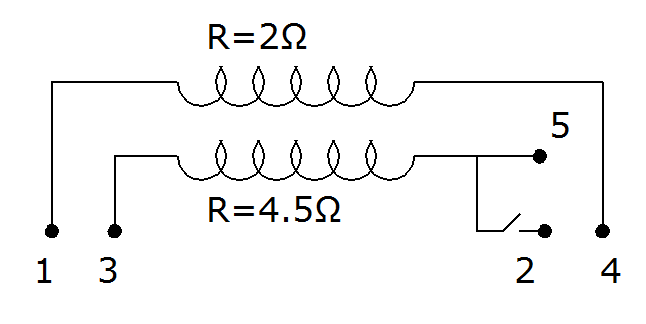
\includegraphics[scale=.5]{dau-day-thuc-te}
\end{center}
\caption{Xác định cực tính của động cơ 1 pha 4 đầu dây}\label{Fig:So-do-ra-day-thuc-tap}
\end{figure}
\begin{list}{--}{}
\item Với động cơ được quấn cho 2 cách khởi động: chạy tụ đề và chạy tụ ngậm thì khi đo giá trị điện trở, cuộn đề sẽ có giá trị điện trở lớn hơn (do số vòng dây nhiều hơn), cuộn chạy sẽ có giá trị điện trở nhỏ hơn.
\item Khi đo ngay dây công tắc thì điện trở là $0 \Omega$.
\item Từ việc đo điện trở $\longrightarrow$ xác định được 2 đầu của một cuộn dây $\longrightarrow$ dựa vào giá trị điện trở $\longrightarrow$ xác định được cuộn đề và cuộn chạy. 
\begin{center}
\begin{tabular}{|c|c|c|}\hline
Vị trí định danh của cuộn dây & $1-4$ & $3 - 5$\\ \hline
Giá trị điện trở $\Omega$ & $2 \Omega$ & $4.5\Omega$\\ \hline
Kết luận & Cuộn chạy & Cuộn đề\\ \hline
\end{tabular}
\end{center}
\end{list}
\newpage
\subsection{Sơ đồ đấu dây động cơ chạy tụ khởi động}
\begin{figure}[!h]
\begin{center}
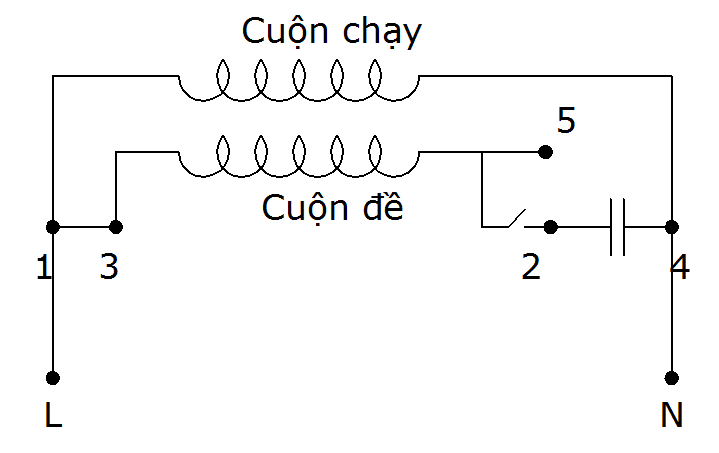
\includegraphics[scale=.4]{dau-day-thuc-te-1}
\end{center}
\caption{Sơ đồ đấu dây động cơ chạy tụ khởi động}\label{Fig:chay-de-1}
\end{figure}
Sau khi đạt được tốc độ, công tắc ly tâm ngắt tụ khởi động và cuộn đề, lúc này chỉ còn cuộn chạy hoạt động.
\subsection{Sơ đồ đấu dây động cơ chạy tụ ngậm}
\begin{figure}[!h]
\begin{center}
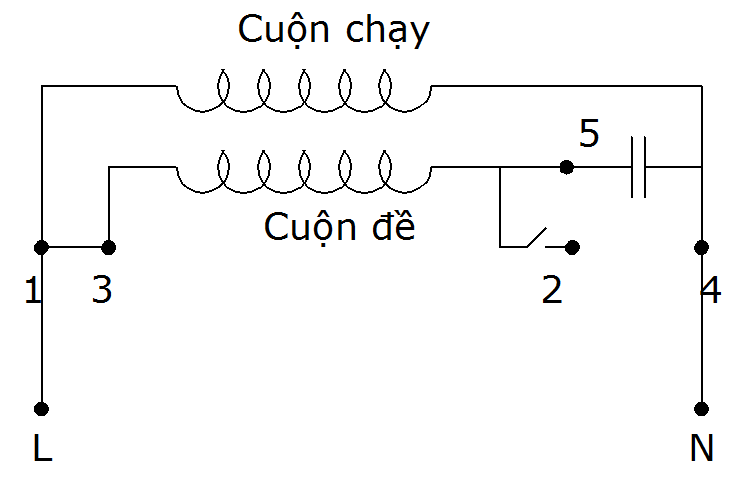
\includegraphics[scale=.4]{dau-day-thuc-te-2}
\end{center}
\caption{Sơ đồ đấu dây động cơ chạy tụ ngậm}\label{Fig:chay-de-11}
\end{figure}
\newpage
\subsection{Mạch động lực và mạch điều khiển đông cơ một pha}
Hai mạch sau sử dụng chung cho động cơ chạy tụ đề và chạy tụ ngậm:
\begin{list}{--}{}
\item Mạch điều khiển như hình~\ref{Fig:mach-dieu-khien-1p-tu-de}.
\begin{figure}[!h]
\begin{center}
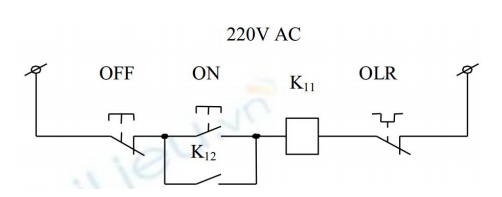
\includegraphics[scale=.6]{van-hanh-1p-tu-de-1}
\end{center}
\caption{Mạch động cơ một pha}\label{Fig:mach-dieu-khien-1p-tu-de}
\end{figure}
\item Mạch động lực như hình~\ref{Fig:mach-dong-luc-1p-tu-de}.
\begin{figure}[!h]
\begin{center}
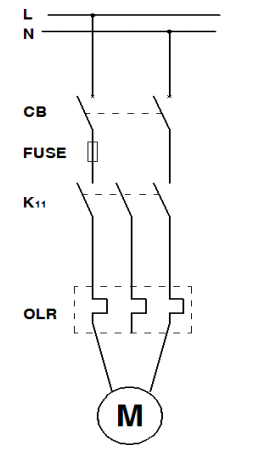
\includegraphics[scale=.6]{van-hanh-1p-tu-de}
\end{center}
\caption{Mạch động lực vận hành động cơ một pha}\label{Fig:mach-dong-luc-1p-tu-de}
\end{figure}
\end{list}
\subsection{Vận hành động cơ một pha ở hai chế độ chạy tụ ngậm và chạy tụ đề}
Kết quả lấy số liệu:
\begin{center}
\begin{tabular}{|c|c|c|c|}\hline
\textit{Động cơ} & $U_{\text{\textit{vận hành}}}, V$ & $I_{\text{\textit{không tải}}}, A$ \\ \hline
Chạy tụ đề & $230$ &$7.3$  \\ \hline
Chạy tụ ngậm & $235$&$5.26$ \\ \hline
\end{tabular}
\end{center}
\subsection{Trả lời câu hỏi}
\paragraph{So sánh động cơ chạy tụ đề và động cơ chay tụ ngậm}
\begin{itemize}
\item \textit{Giống nhau}: đều dùng để tạo từ trường trường quay, moment mở máy cho động cơ hoạt động.
\item \textit{Khác nhau}:
\begin{list}{--}{}
\item Với động cơ chạy tụ đề:
\begin{list}{+}{}
\item Tụ điện chỉ hoạt động lúc khởi động động cơ, sau khi đạt được tốc độ sẽ được ngắt bởi công tắc ly tâm.
\item Mục đích: là tạo từ trường mạnh làm tăng moment khởi động.
\end{list}
\item Với động cơ chạy tụ ngậm: Tụ này sẽ hoạt động trong suốt quá trình hoạt động của động cơ, moment mở máy sẽ nhỏ hơn.
\end{list}
\end{itemize}
\section{Động cơ 3 pha 6 đầu dây}
\subsection{Số liệu trên nhãn của động cơ}
\begin{list}{--}{}
\item Công suất: $P = 1HP = 0.75 kW$.
\item Số cực: 4 cực; tần số $f = 50 - 60Hz$.
\item Hệ số công suất: $SF = 1.0$.
\item Tốc độ quay: $f = 50Hz, n = 1450$ \textit{vòng/phút}; $f = 60Hz, n = 1710$ \textit{vòng/phút}.
\item Điện áp: $220V/380V$.
\item Dòng điện: đấu $Y/\Delta$: $f = 50Hz: I = 3.7/1.8A$ và $f = 60Hz: I = 3.2/1.5A$.
\end{list}
\subsection{Xác định cực tính của động cơ}
Tóm tắt ý tưởng:
\begin{list}{--}{}
\item Từ 6 đầu dây dùng VOM (thang đo $\times 1 \Omega$) để xác định 2 đầu của một cuộn dây. Từ đó xác định được 3 cuộn dây, như chưa xác định được đầu cuối.
\item Dùng pin 9V kết hợp với VOM (thang đo $mA$), một đầu của cuộn dây (giả sử cuộn dây $AX$) $A$ nối vào nguồn $+9V$ đầu còn lại $X$ nối vào $0V$, như trên hình ~\ref{Fig:dau-cuoi-3-pha}.
\item Cuộn dây thứ 2 (giả sử cuộn dây $QP$ thì: que đen $VOM$ vào $Q$ , que đỏ $VOM$ vào $P$, nếu kim quy thuận thì: $QP=BY$, còn quay ngược thì $QP = YB$.
\item Cuộn dây còn lại xác định tương tự như trên.
\begin{figure}[!h]
\begin{center}
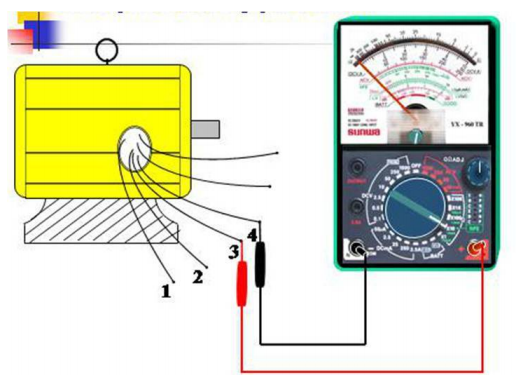
\includegraphics[scale=.5]{VOM-PIN} 
\end{center}
\caption{Cách xác định đầu cuối của động cơ 3 pha}\label{Fig:dau-cuoi-3-pha}
\end{figure}
\end{list}
\newpage
\subsection{Sơ đồ đấu dây động cơ 3 pha kiểu Y}
\begin{figure}[!h]
\begin{center}
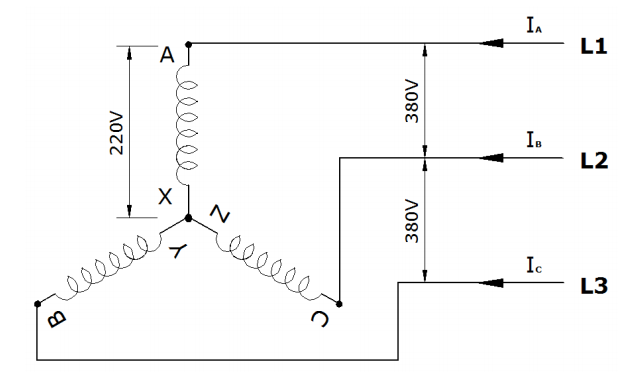
\includegraphics[scale=.5]{dau-day-3-pha-Y.png} 
\end{center}
\caption{Sơ đồ đấu dây động cơ 3 pha kiểu Y}\label{Fig:dc-3p}
\end{figure}
\subsection{Mạch động lực và mạch điều khiển đông cơ ba pha}
\begin{list}{--}{}
\item Mạch điều khiển như hình~\ref{Fig:mach-dieu-khien-3p}.
\begin{figure}[!h]
\begin{center}
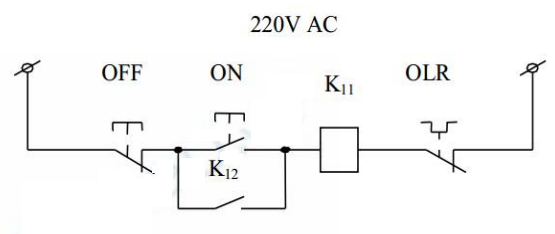
\includegraphics[scale=.6]{van-hanh-3p-1}
\end{center}
\caption{Mạch động cơ ba pha}\label{Fig:mach-dieu-khien-3p}
\end{figure}
\item Mạch động lực như hình~\ref{Fig:mach-dong-luc-3p}.
\begin{figure}[!h]
\begin{center}
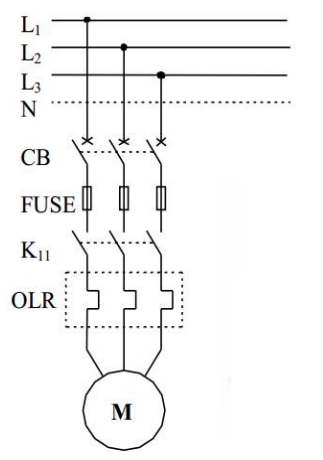
\includegraphics[scale=.6]{van-hanh-3p}
\end{center}
\caption{Mạch động lực vận hành động cơ ba pha}\label{Fig:mach-dong-luc-3p}
\end{figure}
\end{list}
\subsection{Vận hành động cơ 3 pha}
\begin{center}
\begin{tabular}{|c|c|}\hline
$U_{\text{\textit{vận hành}}}, V$ & $I_{\text{\textit{không tải}}}, A$ \\ \hline
$U_{AB} =401.7 $& $I_A = 1.41$ \\ \hline
$U_{BC} =399.1 $& $I_A = 1.26$ \\ \hline
$U_{AC} =404.1 $& $I_A = 1.28$ \\ \hline
\end{tabular}
\end{center}
\section{Câu hỏi ôn tập}
\begin{enumerate}[{\bf 1.}]
\item \textit{Mục đích của việc xác định cực tính của động cơ?}

Là để đấu dây theo sơ đồ đã thiết kế và đưa động cơ vào vận hành.
\item \textit{So sánh động cơ 1 pha và 3 pha. Nêu ứng dụng}
\begin{list}{--}{}
\item Khi cùng một công suất thì động cơ 3 pha khởi động tốt hơn, momen ổn định hơn và hiệu suất cao hơn.
\item Động cơ 3 pha có thể vận hành ở chế độ 1 pha.
\item Động cơ 1 pha có các nhược điểm là hệ số cống suất $\cos \varphi$ thấp, hiệu suất thấp, vì tổn hao ở roto lớn, moment nhỏ nên làm việc kém ổn định, khả năng quá tải kém.
\item Ưu điểm của động cơ điện 1 pha: có cấu tạo gọn, sử dụng điện 1 pha, được dùng nhiều trong tự động, dân dụng (quạt điện, máy giặc, máy bơm nước,\ldots).
\item Với động cơ không đồng bộ 3 pha, khi mở máy cần phải thỏa các điều kiện sau:
\begin{list}{+}{}
\item Moment mở máy của động cơ phải lớn hơn moment tải lúc mở máy.
\item Moment động cơ phải lớn để thời gian mở máy trong phạm vi cho phép.
\item Dòng mở máy phải nhỏ để điện áp lưới không bị sụt áp và không ảnh hưởng đến các thiết bị khác.
\end{list}
\item Động cơ không đồng bộ 3 pha khi khởi động không cần phải dùng tụ (do từ trường biến thiên), ở động cơ không đồng bộ 1 pha khởi động cần đến tụ và cuộn dây phụ (do là từ trường đập mạch, không tạo được từ trường quay).
\item[$\ast$] Ứng dụng:
\begin{list}{+}{}
\item Động cơ 1 pha: thường gặp trong dân dụng, tự động vì sử dụng nguồn 1 pha, công suất sử dụng không lớn.
\item Động cơ 3 pha: thường được dùng trong các nhà máy, các xí nghiệp do có nguồn điện 3 pha để sử dụng, cần công suất lớn, như máy nghiền, máy xoasym\ldots
\end{list}
\end{list}
\item \textit{Phương pháp khởi động trực tiếp có những ưu và khuyển điểm gì. Nêu một số ứng dụng cụ thể?}
\begin{list}{--}{}
\item \textit{Ưu điểm:} Đơn giản, mở máy trực tiếp.
\item \textit{Nhược điểm}: Dòng điện mở máy lớn, nếu quán tính của tải lớn làm cho thời gian mở máy kéo dài, có thể làm cho động cơ phát nóng, ảnh hưởng đến điện áp lưới vì thời gian giảm áp quá lâu, và có thể làm đứt cầu chì bảo vệ.
\item Nếu nguồn điện lớn hơn công suất của động cơ nên dùng phương pháp mở máy trực tiếp vì thời gian mở máy nhanh, phương pháp mở máy đơn giản, moment mở máy lớn.
\item[$\ast$] \textit{Ví dụ}: Các động cơ công suất nhỏ thường sử dụng phương pháp mở máy trực tiếp. Các động cơ công suất lớn thì phải khởi động gián tiếp. $Y/\Delta$.
\end{list}
\item \textit{Hãy nêu một số phương pháp xác định cực tính mà em biết. Nêu ứng dụng cụ thể?}

Ngoài cách xác định như trong bài thực hành (dùng nguồn pin và VOM). Có thể xác định theo 2 cách sao:
\begin{enumerate}[{\it a.}]
\item \textit{Cách 1}: Áp dụng cho trường hợp khi đã biết cực tính của một dây. 
\begin{list}{--}{}
\item Đấu nối tiếp \textit{cuộn dây cần xác định cực tính} vào \textit{cuộn dây đã biết cực tính}.
\item Cấp điện AC vào \textit{cuộn dây đã biết cực tính}.
\item Đo điện thế 2 đầu các cuộn dây: đo 2 đầu cuộn dây đã biết cực tính $U_1$; 2 đầu cuộn dây chưa biết cực tính $U_2$; tổng 2 đầu của 2 cuộn dây này $U$.
\item Nếu $U > U_1 + U_2$: thì 2 cuộn cùng cực tính. Ngược lại $U < |U_1 - U_2|$ thì ngược cực tính.
\end{list}
\item \textit{Cách 2}: Nếu trong điều kiện không có dụng cụ đo, mà tháo được động cơ thì ta nên tháo động cơ ra để quan sát cách đi sơ đồ dây, từ đó xác định được cực tính của các cuộn dây trong động cơ.
\end{enumerate}
\end{enumerate}
\end{document}